\chapter{基于深度学习的点云配准}
本章将结合深度学习,对点云配准进行研究。首先介绍深度学习中点云配准常用的公开数据集,然后介绍点云配准的评价指标并推广到多实例点云配准,最后介绍点云配准相关的深度学习技术。

\section{标准数据集}
本节将介绍用于点云配准的标准数据集。在评估不同指标的性能时,我们需要用到不同的公开数据集。点云配准任务的数据集大致可以分为仿真数据集和真实数据集。仿真数据集中的物体对象是完整的三维模型,比如ModelNet40\cite{sunmodelnet40}。而真实数据集中,因为存在遮挡、测量误差、相干光干扰、背景影响等问题,往往会存在缺失、噪声、过密/稀疏等问题,比如Scan2CAD\cite{avetisyan2019scan2cad}和ShapeNet\cite{chang2015shapenet}。下表\ref{tab:PointCloudDatasets}列出了常用的点云配准数据集。
\begin{table}[h!]
    \centering
    \vspace{-1.0cm}
    \caption{常见的点云信息处理任务数据集列表}
    \label{tab:PointCloudDatasets}
    \resizebox{\textwidth}{!}{
    \begin{tabular}{|l|c|c|c|c|c|c|c|}
    \hline
    \textbf{数据集名称} & \textbf{年份} & \textbf{场景数量} & \textbf{类别数量} & \textbf{训练集} & \textbf{测试集} & \textbf{类型} & \textbf{数据结构} \\ \hline
    McGill Benchmark \cite{siddiqi2008retrieving} & 2008 & 456 & 19 & 304 & 152 & 仿真场景 & 三角网格 \\ \hline
    Sydney Urban Objects \cite{de2013unsupervised} & 2013 & 588 & 14 & - & - & 真实场景 & 点云 \\ \hline
    ModelNet10 \cite{wu20153d} & 2015 & 4899 & 10 & 3991 & 605 & 仿真场景 & 三角网格 \\ \hline
    ModelNet40 \cite{sunmodelnet40} & 2015 & 12311 & 40 & 9843 & 2468 & 仿真场景 & 三角网格 \\ \hline
    ShapeNet \cite{chang2015shapenet} & 2015 & 51190 & 55 & - & - & 仿真场景 & 三角网格 \\ \hline
    ScanNet \cite{dai2017scannet} & 2017 & 12283 & 17 & 9677 & 2606 & 真实场景 & RGB-D \\ \hline
    ScanObjectNN \cite{uy2019revisiting} & 2016 & 2902 & 15 & 2321 & 581 & 真实场景 & 三角网格 \\ \hline
    S3DIS \cite{armeni20163d} & 2017 & 271 & 13 & - & - & 真实场景 & 点云 \\ \hline
    7Scenes \cite{shotton2013scene} & 2013 & 7 & 1 & 26000 & 17000 & 真实场景 & RGB-D \\ \hline
    Scan2CAD \cite{avetisyan2019scan2cad} & 2019 & 1512 & 1 & 1209 & 303 & 真实场景 & 点云 \\ \hline
    \end{tabular}
    }
    \vspace{-1.0cm}
\end{table}

在本次任务中,我们使用ModelNet40、ShapeNet、Scan2CAD组成多实例点云配准仿真数据集进行训练和测试。所以,我们对这3个数据集和多实例点云配准数据集进行了详细的介绍。

\subsection{ModelNet40}
ModelNet 是一个用于三维物体识别和检索的大规模数据集。它包含两个子集:ModelNet10 和 ModelNet40。ModelNet10 包含 10 个类别的 4,899 个模型,而 ModelNet40 包含 40 个类别的 12,311 个模型。ModelNet 数据集中的模型主要是合成的 CAD 模型,并以网格 (mesh) 的形式呈现。本文主要使用 ModelNet40 数据集。 

ModelNet40 主要涵盖了各种常见物体,如办公桌、椅子、沙发、书架、飞机、自行车、花盆等。其中例如杯子、桌子、飞机等这种具有规则对称结构的模型,对于位姿回归、点云配准来说是比较困难的,容易因为对称轴而产生歧义。对于人、花这样具有复杂结构的模型,也很难准确识别模型的关键信息,在点云处理中具有一定的挑战性。ModelNet40 数据集部分可视化结果如图 \ref{fig:modelnet}所示。

\begin{figure}
    \centering
    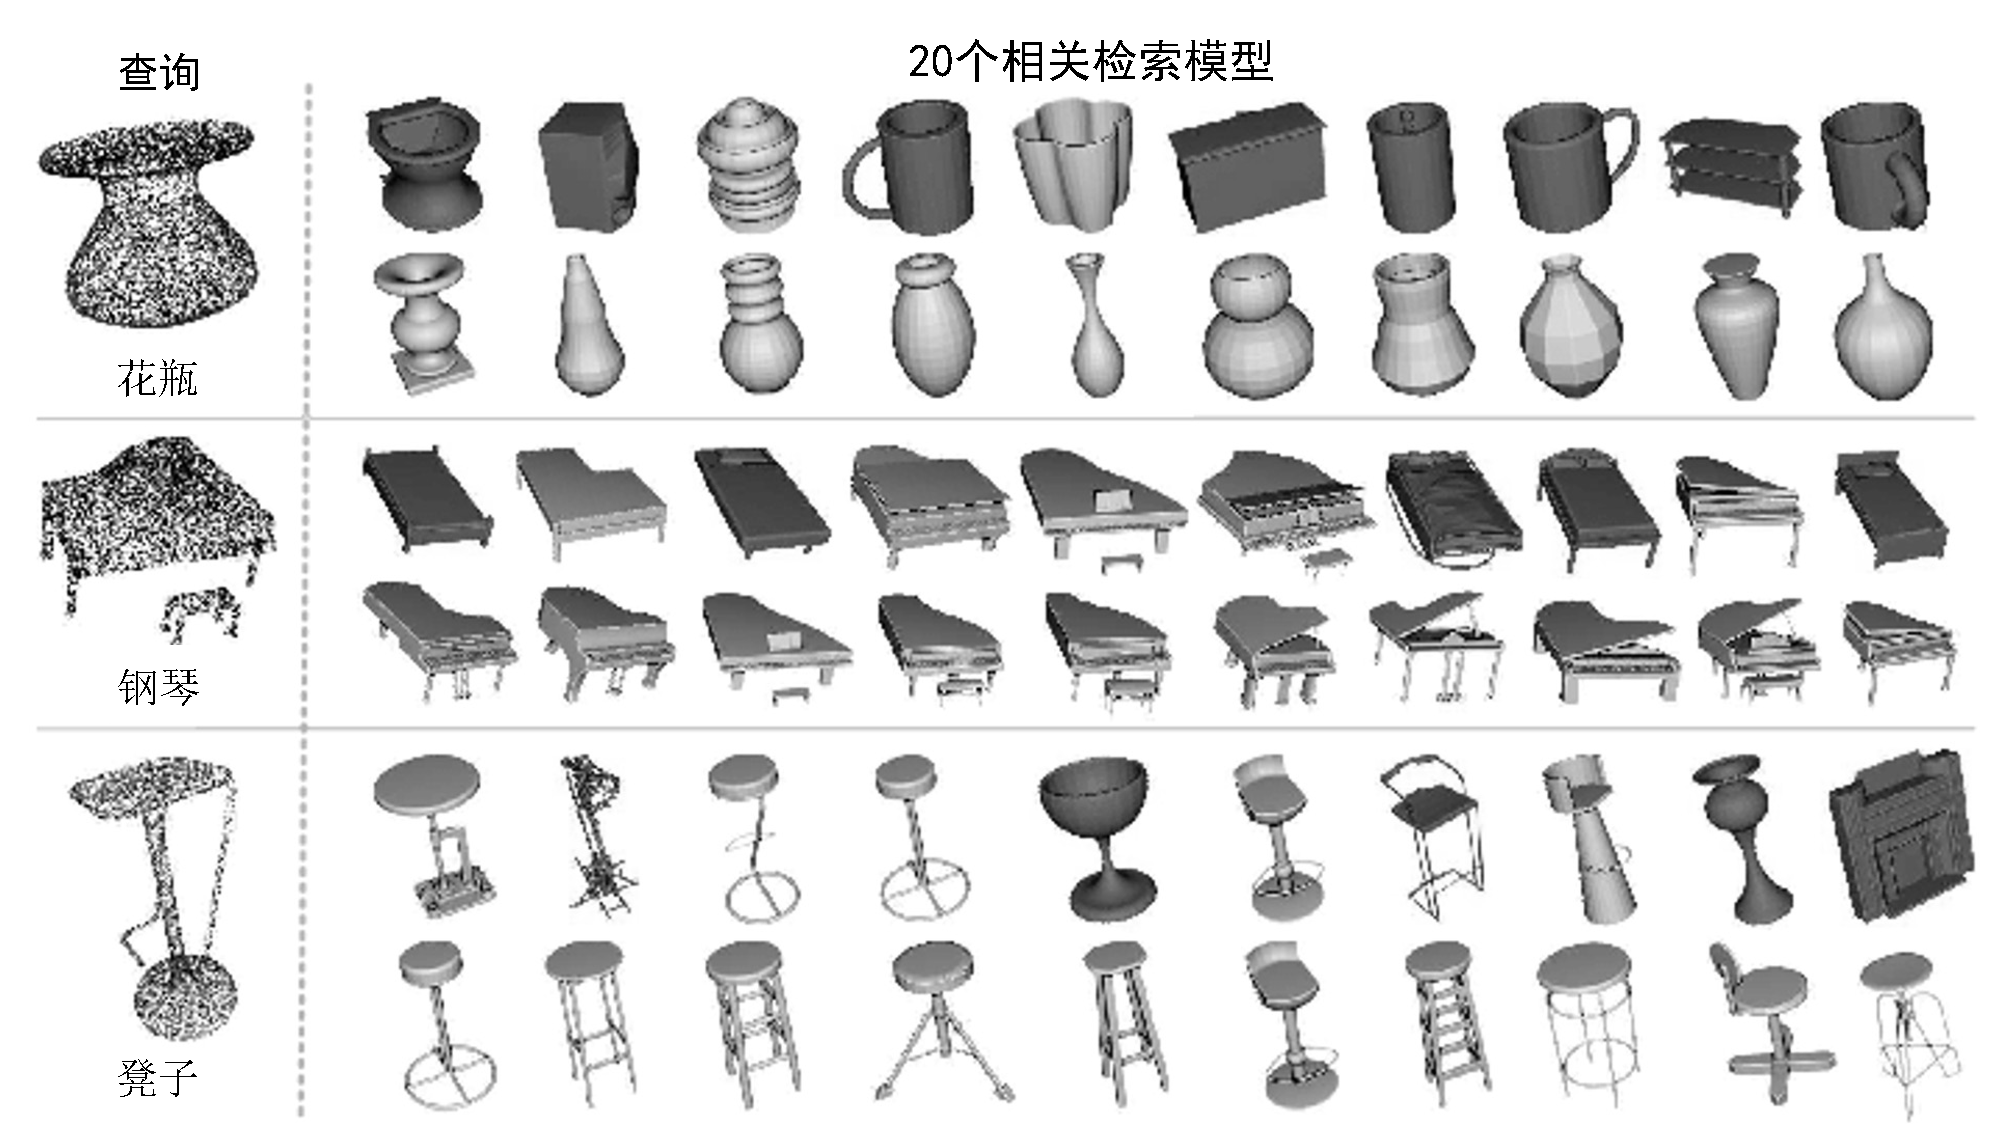
\includegraphics[width=\textwidth]{images/ModelNet.pdf}
    \caption{ModelNet40 数据集部分可视化结果}
    \label{fig:modelnet}
    \vspace{-0.5cm}
\end{figure}

\begin{figure}
    \centering
    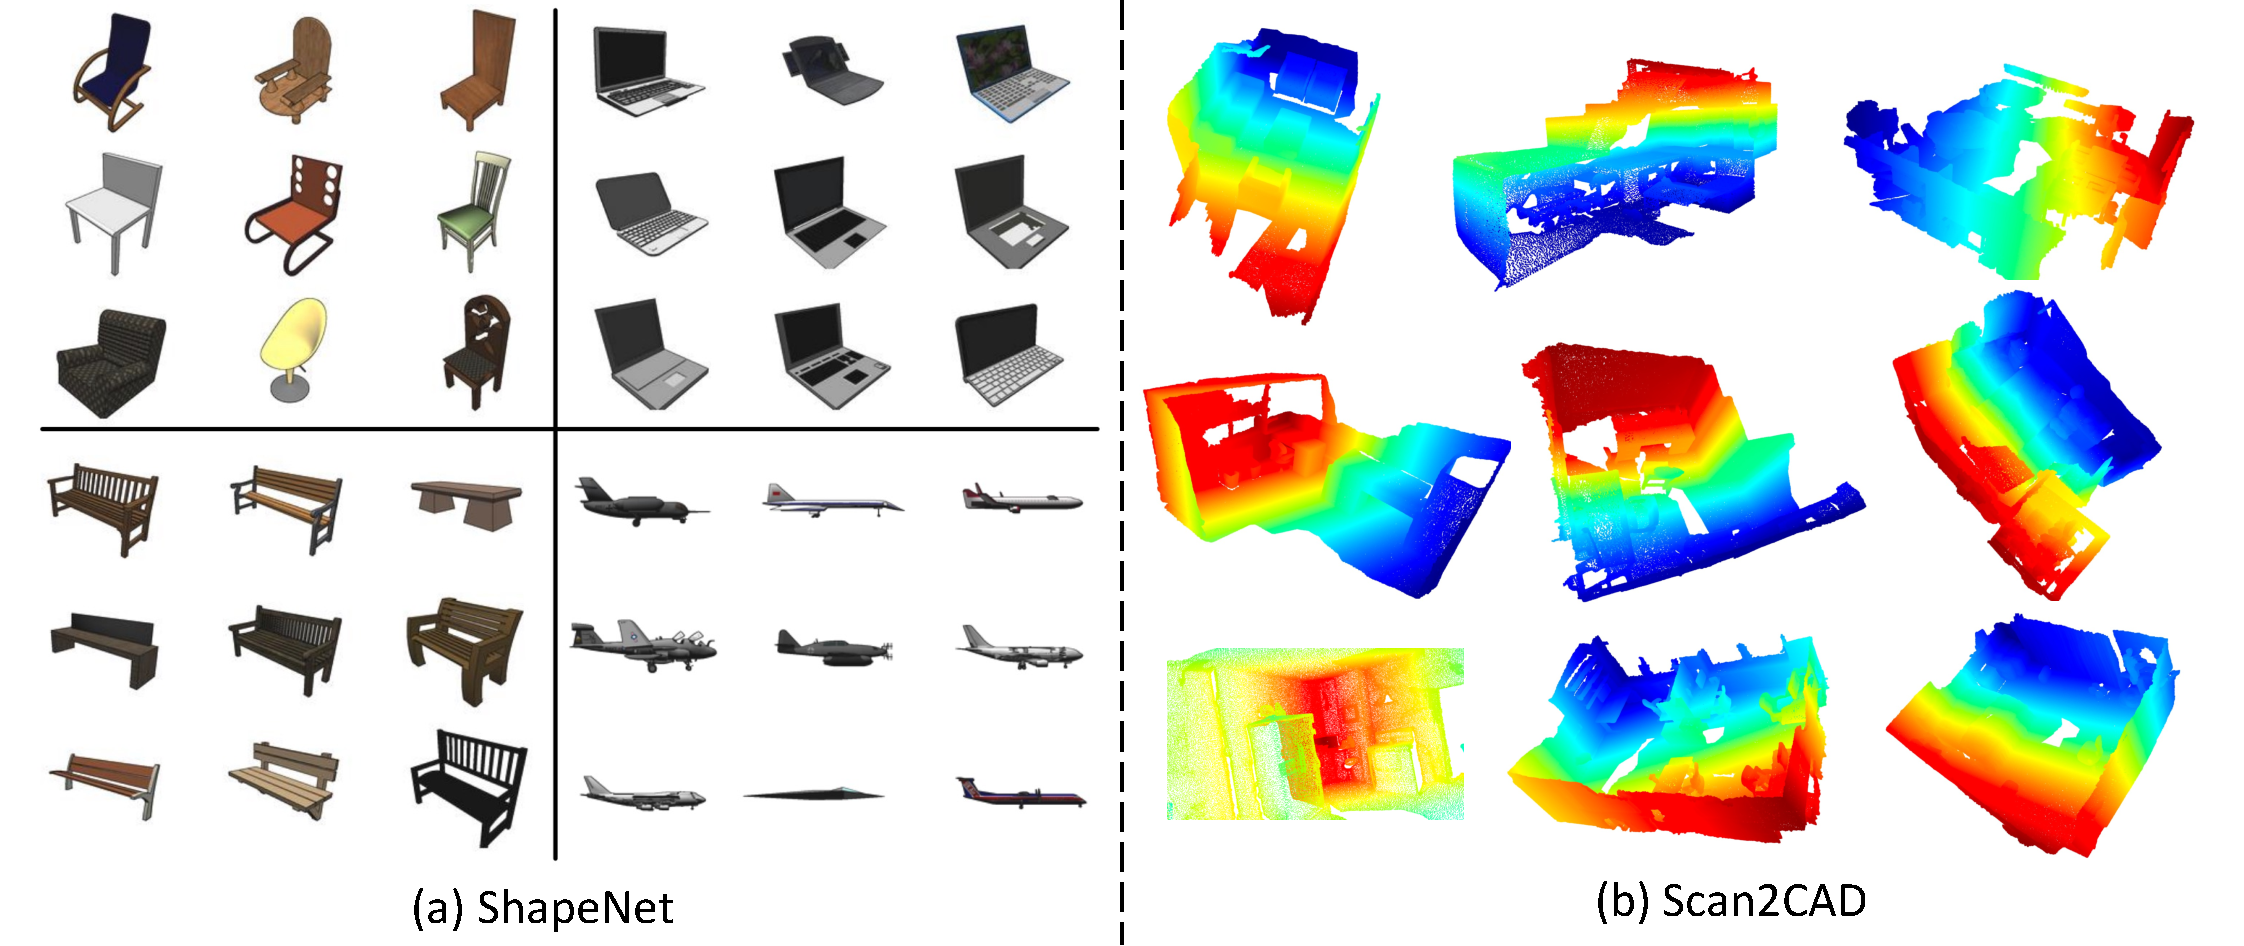
\includegraphics[width=\textwidth]{images/Shapenet-Scan2CAD.pdf}
    \caption{ShapeNet 数据集和Scan2CAD 数据集部分可视化结果}
    \label{fig:ShapeNet&Scan2CAD}
    \vspace{-0.5cm}
\end{figure}
\subsection{ShapeNet}
ShapeNet 数据集是一个大规模的三维模型数据库,其目的是为计算机视觉和图形学领域的研究者提供一个丰富且多样化的数据源。该数据集涵盖了许多不同的物体类别,包括家具、交通工具、家电等。ShapeNet 数据集中的模型具有详细的几何形状和丰富的语义标注,这使得它在多种三维任务中都具有很高的实用价值。

ShapeNet 数据集包含了 55 个类别,共有 51,190 个三维模型。这些模型主要来源于网上的 CAD 模型库,经过清洗和处理后整合成一个统一的数据集。数据集中的每个模型都以网格(mesh)格式存储,并附有与物体相关的语义信息,如类别标签、实例标签等。此外,ShapeNet 数据集还包含了一些额外的元数据,如模型的尺寸、位置和方向等。部分可视化结果如图\ref{fig:ShapeNet&Scan2CAD} (a) 所示。

\subsection{Scan2CAD}
Scan2CAD 数据集是一个用于场景理解和CAD模型对齐的大规模数据集。该数据集的目标是将真实场景的三维扫描与合成的CAD模型相关联。Scan2CAD 数据集包含了从Matterport3D\cite{chang2017matterport3d} 和 ScanNet\cite{dai2017scannet} 等公共数据集中的扫描数据,与来自ShapeNet等数据集的CAD模型。这些扫描和CAD模型之间的对应关系是通过专家注释来确定的。

Scan2CAD 数据集中的扫描数据包含了多种室内场景,如住宅、办公室和公共场所等。这些场景包括了各种物体,如家具、装饰品和建筑元素。与此同时,CAD模型包含了各种详细的几何和拓扑结构。部分可视化结果如图\ref{fig:ShapeNet&Scan2CAD} (b) 所示。

\subsection{多实例点云配准仿真数据集}
数据集:我们在合成数据集和真实数据集上进行实验。我们的合成数据集是从ModelNet40构建的,它包括来自40个类别的12311个网格化CAD模型。为了构建我们的合成数据集,对于每个模型,我们从中均匀地下采样1024个点以形成源点云,然后将其旋转和平移5-10次以生成多个实例。这些实例与噪声点混合,形成如图3所示的目标点云。沿每个轴的旋转在[0,180°]内均匀采样,平移在[0,5]内。我们为合成数据集生成的输入对应关系是通过将真实对应关系与异常值混合而生成的。我们将每个实例的内点比率控制在约2\%。我们使用12311个模型生成了12311个这样的合成源-目标点云对。我们使用9843对进行训练,2468对进行测试。我们在训练集中随机留出10\%的对作为验证集。

\subsection{多实例点云配准真实数据集}
我们的真实数据集是 Scan2CAD ,它利用 ShapeNet 和 ScanNet 构建而成。此数据集使用 ShapeNet 中的 CAD 模型替换真实扫描场景中的点云,并提供精确的注释,包括模型类别、旋转和平移等。数据集提供了 1506 个带注释的场景,每个场景至少包含一个实例类别。因此,我们充分利用这些注释,并将包含多种实例的场景分割成多个源-目标点云对,用于多实例注册。通过这种方式,我们得到了 2184 对点云,其中大多数点云在目标点云中包含 2-5 个相同类别的实例。我们按照 7:1:2 的比例将样本划分为训练集、验证集和测试集。我们使用微调的 FCGF\cite{FCGF2019} 生成局部特征并通过特征匹配生成假设的对应关系。
\begin{table}[h]
    \centering
    \vspace{-1.0cm}
    \begin{minipage}{0.45\textwidth}
        \centering
        \caption{FCGF 网络参数设置和预训练}
        \label{tab:fcgf}
        \begin{tabular}{cc}
        \toprule
        \multicolumn{2}{c}{FCGF 网络参数设置和预训练} \\ 
        \midrule
        模型                 & RESUNETBN2C      \\ 
        下采样体素大小          & 2.5cm (0.025)    \\ 
        特征维度                & 32               \\ 
        预训练数据集             & 3DMatch          \\ 
        特征归一化              & 是               \\ 
        \bottomrule
        \end{tabular}
    \end{minipage}
    \hfill
    \begin{minipage}{0.45\textwidth}
        \centering
        \caption{FCGF 网络微调参数设置}
        \label{tab:fcgf_finetune}
        \begin{tabular}{cc}
        \toprule
        \multicolumn{2}{c}{FCGF 网络微调参数设置} \\ 
        \midrule
        批量大小               & 4                 \\ 
        学习率                 & $10^{-3}$         \\ 
        迭代次数                & 20                \\ 
        优化器                 & SGD               \\ 
        \bottomrule
        \end{tabular}
    \end{minipage}
    \vspace{-1.0cm}
\end{table}

这里,我们主要关注如何通过特征匹配生成假设的对应关系。我们使用 FCGF 作为特征提取器,参数设置如表 \ref{tab:fcgf} 所示。FCGF 网络在 3DMatch 数据集上预训练,然后使用表 \ref{tab:fcgf_finetune} 中的参数设置进行微调。微调过的 FCGF 提取 L2归一化的局部特征 $F_{local}^X = \{f_{local}^{x_i} \in \mathbb{R}^{32} | i = 1, \dots, |X|\}$,用于源点云 $X$ 和 $F_{local}^Y = \{f_{local}^{y_i} \in \mathbb{R}^{32} | i = 1, \dots, |Y|\}$,用于目标点云 $Y$,其中 $|X|$ 和 $|Y|$ 分别表示源点云和目标点云中的点数。给定目标点云 $Y$ 中的每个点 $y_j$,我们找到满足 $i = \arg\max_i \langle f_{local}^{y_j}, f_{local}^{x_i} \rangle$ 的源点云 $X$ 中的点 $x_i$ 以构建对应关系 $(x_i, y_j)$,其中 $\langle f_{local}^{y_j}, f_{local}^{x_i} \rangle$ 是两点特征之间的余弦相似度。这样,我们获得 $|Y|$ 个对应关系,我们将余弦相似度 $\langle f_{local}^{x_i}, f_{local}^{y_j} \rangle$ 定义为对应关系 $(x_i, y_j)$ 的显著性得分。我们选择显著性得分最大的 $K$ 个对应关系,然后将这些 $K$ 个对应关系随机下采样为 $N$ 个对应关系作为输入的假设对应关系。这里,我们将 $K$ 设置为 10000,以使输入对应关系尽可能覆盖更多实例。
\section{点云配准评价指标}
对于配准任务,评估指标可以主要分为两类,一类是用于特征提取与匹配的评价指标,另一类是用于配准结果运动参数评价的指标。
\subsection{基于特征提取与匹配的评价指标}
\subsubsection{特征匹配召回率 (Feature Matching Recall)}
特征匹配召回率衡量了匹配算法在正确提取匹配点对数量和所有点对数量之间的比率,反映了匹配算法的查全率。从数学角度来看,特征匹配召回率可以表示为:
\begin{equation}
R_{fa} = \frac{1}{n} \sum_{s=1}^{n} \mathbbm{1} \left( \frac{1}{|\boldsymbol{\omega}|} \sum_{(\boldsymbol{i},\boldsymbol{j})\in\boldsymbol{\omega}} (\lVert \boldsymbol{T}\boldsymbol{p}_i - \boldsymbol{q}_j \rVert < \tau_1) > \tau_2 \right)
\end{equation}
其中 $n$ 是所有点对的数量,$\boldsymbol{\omega}$ 是匹配点对 $(\boldsymbol{p}, \boldsymbol{q})$ 之间的对应关系集合,$\boldsymbol{p} = (x_p, y_p, z_p)$,$\boldsymbol{q} = (x_q, y_q, z_q)$,$\boldsymbol{T} \in SE(3)$ 是地面真实姿态变换矩阵。此外,$\tau_1$ 是内部距离阈值,$\tau_2$ 是内部召回率阈值。
\subsubsection{点云配准召回率 (Point Cloud Registration Recall)}
配准召回率衡量了在具有地面真实姿态变换且存在重叠部分的两组点云中,有多少重叠部分的点云组可以通过匹配算法被正确恢复。具体而言,配准召回率使用如下误差矩阵来定义真阳性:
\begin{equation}
    E = \sqrt{\frac{1}{|\boldsymbol{\omega}^*|} \sum_{(\boldsymbol{p}^*,\boldsymbol{q}^*)\in\boldsymbol{\omega}^*} \lVert \boldsymbol{\hat{T}}_{i,j}\boldsymbol{p}^* - \boldsymbol{q}^* \rVert^2} < \tau_3
\end{equation}
    
其中,$\boldsymbol{\omega}^*$ 是重叠部分一组匹配点对 $(\boldsymbol{p}^*, \boldsymbol{q}^*)$ 之间的对应关系集合,$\boldsymbol{p}^* = (x^*_p, y^*_p, z^*_p)$,$\boldsymbol{q}^* = (x^*_q, y^*_q, z^*_q)$。对于重叠部分,$\tau_3$ 是用于判断匹配点对是否正确的阈值。

\subsection{基于刚体运动的评价指标}
\subsubsection{投影的均方根误差}
投影的均方根误差 (RMSE Projection) 是在应用变换之后,计算点到点投影误差的平均值。计算公式为:
\begin{equation}
    \text{RMSE} (\boldsymbol{p}) = \frac{1}{n}\sum_{i=1}^{n} \sqrt{(\boldsymbol{p}_i^{'} - \boldsymbol{p}_i)^2},
\end{equation}
其中 $n$ 是点云中的点数,$\boldsymbol{p}_i^{'}$ 是应用变换后的点,$\boldsymbol{p}_i$ 是原始点。

\subsubsection{变换的均方根误差}
变换的均方根误差 (RMSE Tranformation) 代表估计的变换 $\boldsymbol{\hat{T}}_{s}$ 和真实变换 $\boldsymbol{T}^*_{s}$ 之间的均方根误差。计算公式为:
\begin{equation}
    \text{RMSE} (\boldsymbol{T}) = \sqrt{\frac{1}{n}\sum_{i=1}^{n}(\boldsymbol{\hat{T}}_{s} - \boldsymbol{T}^*_{s})^2},
\end{equation}

\subsubsection{相对旋转误差}
我们定义相对旋转误差 (Relative Rotation Error) 为真实变换 $\boldsymbol{T}^*_{s}$ 和估计变换 $\boldsymbol{\hat{T}}_{s}$ 之间的旋转误差。计算公式为:
\begin{equation}
    \text{RRE}_s = \arccos \left(\frac{\operatorname{tr}(\boldsymbol{\hat{R}}_{s} \boldsymbol{R}^*_s) - 1}{2}\right),
\end{equation}
其中 $\operatorname{tr}$ 表示矩阵的迹(对角线元素之和),$\boldsymbol{\hat{R}}_{s}$ 和 $\boldsymbol{R}^*_s$ 分别表示估计变换和真实变换的旋转矩阵。

\subsubsection{相对平移误差}
我们定义相对平移误差 (Relative Transition Error) 为真实变换 $\boldsymbol{T}^*_s$ 和估计变换 $\boldsymbol{\hat{T}}_{s}$ 之间的平移误差。计算公式为:
\begin{equation}
    \text{RTE}_s = \lVert \boldsymbol{t}^*_s - \boldsymbol{\hat{t}}_{s} \rVert,
\end{equation}
其中 $\boldsymbol{t}^*_s$ 和 $\boldsymbol{\hat{t}}_{s}$ 分别表示真实变换和估计变换的平移向量。

\subsection{多实例点云配准评价指标}
\label{sec:multiinstance_eval}
用于评估多实例点云配准性能的三个指标分别是平均命中召回率、平均命中精度和平均命中 F1 分数。

\subsubsection{平均命中召回率 (Mean Hit Recall)}
平均命中召回率衡量了正确恢复的点云对数占所有点云对数的比例。平均命中召回率 (Mean Hit Recall) 在两个已配准的点云之间的定义如下:
\begin{equation}
    \text{MHR} = \frac{1}{\boldsymbol{K}} \sum_{s=1}^{S} \boldsymbol{I}_s
\end{equation}
其中 $\boldsymbol{I}_s = {0, 1}$ 表示一个真实估计对是否为“命中”。具体而言,
\begin{equation}
    \boldsymbol{I}_s = \boldsymbol{I}(\text{RRE}_s < \tau_r) \times \boldsymbol{I}(\text{RTE}_s < \tau_t)
\end{equation}
其中 $\boldsymbol{I}(\cdot) = {0, 1}$ 表示一个指示函数。$\text{RRE}_s$ 和 $\text{RTE}_s$ 是第 $s$ 个真实估计对的相对旋转误差和相对平移误差。两个阈值 $\boldsymbol{\tau_r}$ 和 $\boldsymbol{\tau_t}$ 分别设置为 $20^\circ$ 和 $0.5m$。通过对所有点云对的 \text{MHR} 求平均值,得到最终的平均命中召回率。

\subsubsection{平均命中精确度 (\text{Mean Hit Precision})}
两个已配准的点云之间的平均命中精确度定义如下:

\begin{equation}
\text{MHP} = \frac{1}{\boldsymbol{M}} \sum_{s=1}^{S} \boldsymbol{I}_s
\end{equation}
通过对所有点云对的 \text{MHP} 求平均值,得到最终的平均命中精确度。

\subsubsection{平均命中 F1 (\text{Mean Hit F1})}
两个已配准的点云之间的平均命中 F1 定义如下:
\begin{equation}
\text{MHF1} = \frac{2 \times \text{MHP} \times \text{MHR}}{\text{MHP} + \text{MHR}}
\end{equation}
通过对所有点云对的 \text{MHF1} 求平均值,得到最终的平均命中 F1。


\section{点云处理与配准相关深度学习技术}

\subsection{深度学习概述}
在过去的十年中,深度学习在计算机视觉、自然语言处理等各个领域取得了重要进展 \cite{lecun2015deep}。随着激光雷达、RGB-D 相机和其他三维扫描设备获取的 3D 数据日益增多,深度学习技术逐渐应用于点云处理任务,包括点云配准 \cite{wang2019dynamic, choy2020deep}。点云配准是 3D 计算机视觉中的一个基本问题,目的是找到将两个点云精确对齐的最优变换。

近年来,针对点云配准的深度学习方法已经在自动学习区分性特征和从大规模数据集中学习鲁棒匹配策略方面展示出优于传统方法的性能 \cite{huang2022multiway, lu2019deepvcp}。这些方法利用各种类型的网络架构,例如 PointNet \cite{qi2017pointnet}、PointNet++ \cite{qi2017pointnet++} 和 DGCNN \cite{wang2019dynamic},有效地处理点云数据的非结构化和无序特性。

训练深度神经网络涉及使用反向传播算法,该算法通过应用链式法则计算损失函数相对于每个权重的梯度。使用基于梯度的优化方法(如随机梯度下降(SGD)、Adam\cite{kingma2014adam} 或 MoCo\cite{he2020momentum})更新权重。为了防止过拟合,采用了如 dropout 等正则化技术,即在训练过程中随机将一层中的一部分神经元设置为零。这种策略迫使网络学习更鲁棒的特征,提高了对未见数据的泛化能力。

\begin{equation}
    L(\boldsymbol{W}) = \frac{1}{N} \sum_{i=1}^{N} L_i(\boldsymbol{W}) + \lambda \sum_{l=1}^{L} \lVert \boldsymbol{W}^{(l)} \rVert^2
\end{equation}

在上述方程中,$L(\boldsymbol{W})$ 表示总损失,$L_i(\boldsymbol{W})$ 表示第 $i^{th}$ 个样本的损失,$\boldsymbol{W}^{(l)}$ 表示第 $l$ 层的权重,$L$ 是总层数,$\lambda$ 是正则化参数,$\lVert \cdot \rVert^2$ 表示平方 Frobenius 范数。

为了方便设计、训练和部署深度学习模型,开发了几种深度学习框架,包括TensorFlow\cite{abadi2016tensorflow}、PyTorch\cite{paszke2019pytorch}、PaddlePaddle\cite{ma2019paddlepaddle} 和 MXNet\cite{chen2015mxnet}。这些框架提供了神经网络层、优化算法和其他实用工具的高效实现,使设计、训练和部署深度学习模型变得更加容易。此外,它们还支持使用 GPU (torch.cuda)或专用加速器(如 TPU)进行硬件加速,以加快训练过程。
\subsection{多层感知机}
多层感知器(Multilayer Perceptron, MLP)是一种广泛应用于各种机器学习任务的前馈神经网络\cite{lecun2015deep}。MLP 的基本结构包括输入层、一个或多个隐藏层和输出层。每一层由若干个神经元组成,相邻层的神经元之间通过权重连接。通常,MLP 采用全连接结构,即每个神经元都与上一层和下一层的所有神经元连接。

在训练 MLP 时,需要先进行前向传播计算,即从输入层到输出层计算预测值。接下来,通过反向传播算法计算损失函数对权重的梯度。最后,使用梯度下降或其变体更新权重。

考虑一个简单的两层 MLP,其输入层有 $n$ 个神经元,输出层有 $m$ 个神经元。对于输入向量 $\boldsymbol{x} \in \mathbb{R}^{n}$ 和权重矩阵 $\boldsymbol{W} \in \mathbb{R}^{m \times n}$,MLP 的输出为:

\begin{equation}
\boldsymbol{y} = f(\boldsymbol{W}\boldsymbol{x} + \boldsymbol{b}),
\end{equation}

其中 $\boldsymbol{b} \in \mathbb{R}^{m}$ 是偏置向量,$f$ 是激活函数。在实际应用中,激活函数通常为非线性函数,如 Sigmoid、ReLU 或 Tanh。这些非线性激活函数使得 MLP 能够捕捉复杂的非线性关系。

现在我们考虑一个具有 $L$ 个隐藏层的 MLP,设第 $l$ 层的权重矩阵为 $\boldsymbol{W}^{(l)} \in \mathbb{R}^{n_l \times n_{l-1}}$,偏置向量为 $\boldsymbol{b}^{(l)} \in \mathbb{R}^{n_l}$,激活函数为 $f^{(l)}$。前向传播过程可表示为:

\begin{equation}
\boldsymbol{a}^{(l)} = f^{(l)}(\boldsymbol{W}^{(l)}\boldsymbol{a}^{(l-1)} + \boldsymbol{b}^{(l)}),
\end{equation}

其中 $\boldsymbol{a}^{(0)} = \boldsymbol{x}$,$\boldsymbol{a}^{(L)} = \boldsymbol{y}$。对于损失函数 $L(\boldsymbol{y}, \boldsymbol{t})$,其中 $\boldsymbol{t}$ 是目标输出,我们使用梯度下降方法优化权重和偏置:

\begin{equation}
\boldsymbol{W}^{(l)} \leftarrow \boldsymbol{W}^{(l)} - \alpha \frac{\partial L}{\partial \boldsymbol{W}^{(l)}}, \\
\end{equation}
\begin{equation}
\boldsymbol{b}^{(l)} \leftarrow \boldsymbol{b}^{(l)} - \alpha \frac{\partial L}{\partial \boldsymbol{b}^{(l)}},
\end{equation}

其中 $\alpha$ 是学习率。

为了计算梯度,我们使用反向传播算法。首先,计算输出层关于损失函数的梯度:

\begin{equation}
\boldsymbol{\delta}^{(L)} = \frac{\partial L}{\partial \boldsymbol{a}^{(L)}} \odot f'^{(L)}(\boldsymbol{W}^{(L)}\boldsymbol{a}^{(L-1)} + \boldsymbol{b}^{(L)}),
\end{equation}

其中 $\odot$ 表示哈达玛积(元素对应相乘),$f'^{(L)}$ 是激活函数的导数。

然后,我们从输出层向输入层反向计算梯度:

\begin{equation}
\boldsymbol{\delta}^{(l)} = \left( \boldsymbol{W}^{(l+1)} \right)^T \boldsymbol{\delta}^{(l+1)} \odot f'^{(l)}(\boldsymbol{W}^{(l)}\boldsymbol{a}^{(l-1)} + \boldsymbol{b}^{(l)}).
\end{equation}

最后,我们计算损失函数关于权重和偏置的梯度:

\begin{equation}
\frac{\partial L}{\partial \boldsymbol{W}^{(l)}} = \boldsymbol{\delta}^{(l)} \left( \boldsymbol{a}^{(l-1)} \right)^T, \\
\end{equation}
\begin{equation}
\frac{\partial L}{\partial \boldsymbol{b}^{(l)}} = \boldsymbol{\delta}^{(l)}.
\end{equation}

在实际应用中,为了提高训练速度和泛化能力,我们通常采用 mini-batch 随机梯度下降或其变体(如 Adam、RMSprop 等)进行训练。此外,我们还可以使用正则化技术(如 L1、L2正则化、Dropout 等)防止过拟合。在深度学习框架(如 TensorFlow、PyTorch、PaddlePaddle 和 MXNet 等)的支持下,我们可以方便地实现和训练 MLP 模型\cite{lecun2015deep}。

MLP 是深度学习领域的一个基本概念,尽管现在有许多更复杂的神经网络结构(如卷积神经网络、循环神经网络和 Transformer 等)已经在各种任务上表现出更好的性能,但 MLP 仍然是一个重要的基础知识。通过学习 MLP 的基本原理,我们可以更好地理解神经网络的工作原理,从而有助于设计更复杂的模型和解决更高级的问题。

在实际应用中,MLP 可以处理各种类型的数据,如图像、文本、语音和其他结构化或非结构化数据。由于 MLP 可以近似任意连续函数,因此具有很强的表达能力。然而,MLP 也存在一些局限性。首先,MLP 的参数数量随着层数和每层神经元数量的增加而快速增长,这可能导致过拟合和计算效率低下的问题。其次,MLP 对输入数据的缩放和平移具有较强的敏感性,因此需要对输入数据进行预处理,如归一化。此外,MLP 并不能直接处理变长输入数据和序列数据,需要采用其他神经网络结构,如循环神经网络(RNN)。

尽管如此,MLP 作为一种基础的神经网络结构,在许多任务中仍具有竞争力。例如,在监督学习任务中,MLP 可以用于分类和回归问题;在无监督学习任务中,MLP 可以用于降维和聚类。通过合适的设计和训练策略,MLP 能够在各种应用场景中实现良好的性能。

总之,多层感知器(MLP)是深度学习领域的一个基本概念,作为前馈神经网络的一种,它具有广泛的应用价值。MLP 主要包括输入层、隐藏层和输出层,通过前向传播、反向传播算法进行训练。
\subsection{卷积神经网络}
卷积神经网络(CNN)是一类在各种任务中取得显著成功的深度学习模型,尤其在图像识别、目标检测和自然语言处理等领域。CNN 旨在学习空间特征层次结构,使其特别适用于处理网格状数据(如图像),其中局部依赖关系至关重要\cite{chua1993cnn}。

CNN 的基本构建模块是卷积层。在这个层中,小滤波器(也称为内核)应用于输入,计算滤波器和输入之间的局部点积。这个操作生成一个特征映射,对输入和滤波器之间的空间关系进行编码\cite{he2016deep}。滤波器权重在训练过程中学习,使网络能够自动学习任务特定特征。

从数学上讲,CNN 中的卷积运算可以描述为以下形式:

\begin{equation}
  y_{i,j} = \sum_{m} \sum_{n} x_{i-m, j-n} \cdot w_{m,n},
\end{equation}

其中 $x$ 是输入,$w$ 是滤波器,$y$ 是输出特征映射,$i$、$j$、$m$ 和 $n$ 是输入和滤波器的空间维度对应的索引。

CNN 的一个关键方面是在整个输入中使用共享权重。这种参数共享显著减少了可训练参数的数量,使模型比全连接网络更具计算效率且不容易过拟合。此外,它使网络能够学习平移不变特征,因为相同的滤波器应用于输入的不同空间位置。

CNN 中的另一个重要组件是池化层,用于减少特征映射的空间尺寸。池化层通常在一个或多个卷积层之后应用,以实现局部平移不变性并减少网络的计算复杂性。有不同类型的池化操作,如最大池化、平均池化和全局池化。最大池化是最常用的池化方法,可以定义为:

\begin{equation}
  z_{i,j} = \max_{m,n \in P} x_{i+m, j+n},
\end{equation}

其中 $x$ 是输入特征映射,$z$ 是池化后的输出,$P$ 是池化窗口,$i$、$j$、$m$ 和 $n$ 是输入和池化窗口的空间维度对应的索引。

除了卷积和池化层之外,CNN 通常包括一个或多个全连接层,对学习到的特征进行高级推理。最后一个全连接层的输出通常通过 softmax 激活函数传递,以生成任务特定类别的概率。整个网络使用反向传播和基于梯度的优化算法(如随机梯度下降或 Adam)进行训练。

CNN 已成功应用于广泛的任务,包括图像分类、目标检测、语义分割和自然语言处理。CNN 的成功可以归因于其学习输入数据的分层表示、共享权重和平移不变特征的能力。此外,通过修改其架构和损失函数,CNN 可以轻松地适应不同的任务\cite{albawi2017understanding}。

\subsection{注意力机制}
注意力机制已经成为深度学习模型的重要组成部分,特别是在计算机视觉和点云处理任务中。注意力机制的核心概念是让模型在处理输入数据时,根据上下文信息有选择地关注不同部分,从而提高性能和可解释性。

在计算机视觉领域,注意力机制可以帮助模型更有效地识别和关注图像中的重要区域,以实现更准确的对象识别、语义分割和目标检测。在点云处理任务中,注意力机制可以帮助模型学习点云中的局部和全局结构特征,从而在点云配准、点云分割和分类任务中实现更高的性能。

数学上,注意力机制可以通过以下方式进行描述:

\begin{equation}
\text{Attention}(\boldsymbol{Q}, \boldsymbol{K}, \boldsymbol{V}) = \text{softmax}(\frac{\boldsymbol{Q}\boldsymbol{K}^\top}{\sqrt{d_k}})\boldsymbol{V},
\end{equation}

其中 $\boldsymbol{Q}$、$\boldsymbol{K}$ 和 $\boldsymbol{V}$ 分别表示查询(Query)、键(Key)和值(Value)矩阵,$d_k$ 是键和查询向量的维度。这个计算过程可以解释为:查询向量与键向量的点积表示它们之间的相似性,通过应用 softmax 函数将这些相似性归一化为概率分布,然后使用这些概率分布加权值向量,得到最终的输出。

在计算机视觉和点云处理任务中,注意力机制通常与卷积神经网络(CNN)或图神经网络(GNN)结合使用,以捕获局部和全局上下文信息。这些组合模型在大量基准数据集上表现出卓越的性能,证明了注意力机制在这些领域的有效性。


\section{基于深度学习的点云配准方法}
本节主要阐述主要的基于深度学习的点云配准方法作为基准线,主要阐述PointNet\cite{qi2017pointnet, qi2017pointnet++}系列框架、Predator\cite{huang2021predator}描述子和TEASER\cite{yang2020teaser}配准方法。

\subsection{PointNet \& PointNet++}
\begin{figure}
    \centering
    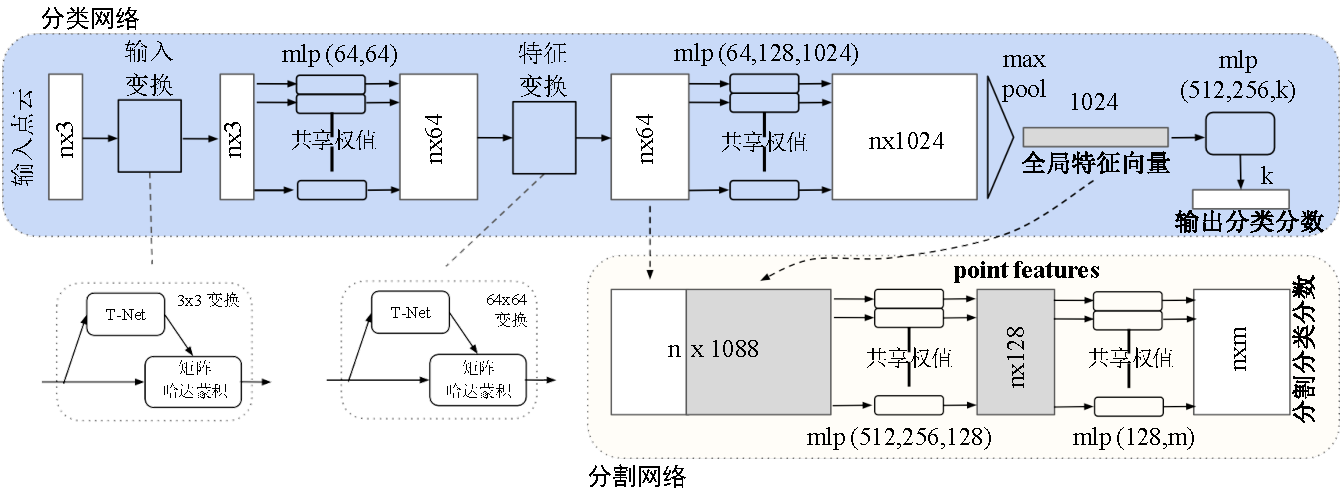
\includegraphics[width=\linewidth]{images/pointnet.pdf}
    \caption{PointNet\cite{qi2017pointnet}网络结构图}
    \label{fig:pointnet}
    \vspace{-5mm}
\end{figure}

\subsubsection{PointNet}
点云处理任务中,我们首先可以朴素地想到直接用多层感知机\cite{lecun2015deep}对作为点云的输入,但是这样的方法对于$N$个点云来说,需要$N \times 3$大小的输入维度,点云数量多时,对于多层感知机过于庞大。所以PointNet提出,对于输入点云,采用共享权值的MLP进行特征提取
\begin{equation}
    \boldsymbol{f_p}_i = f(\theta; \boldsymbol{p}_i)
\end{equation}
然后对特征进行特征变换,对于变换后的特征再次进行升维操作,最终通过$n$个点云数据,得到$n \times 1024$的特征图。将特征图进行最大吃池化操作,得到全局特征向量。

对于分类任务,每一个点云对应一个类别,所以全局特征可以直接用来判断类别信息,通过一个MLP输出最终的分类分数,达到分类的效果。对于点云分割任务,全局特征不足以描述分割的模式,需要加入局部特征。所以将全局特征向量和$\boldsymbol{f_p}_i$进行拼接操作,得到局部+全局特征,通过MLP输出分割的分类分数。

\subsubsection{PointNet++}
PointNet++\cite{qi2017pointnet++}则在PointNet上做了改进。前文提到的PointNet在点云处理中有一个重大缺陷,即点云是具有丰富的表面几何特征的数据格式,也就是说,每一个点都和周围的点产生了交互,但是PointNet仅仅提取出了点的特征和全局特征,缺失了提取局部特征这一过程。这在训练神经网络的时候,往往会导致模型的泛化能力有限\cite{qi2017pointnet++}。所以PointNet++对此作出了调整,在PointNet的基础上提去了不同尺度的局部特征,图示如图\ref{fig:pointnet++}。

\begin{figure}
    \centering
    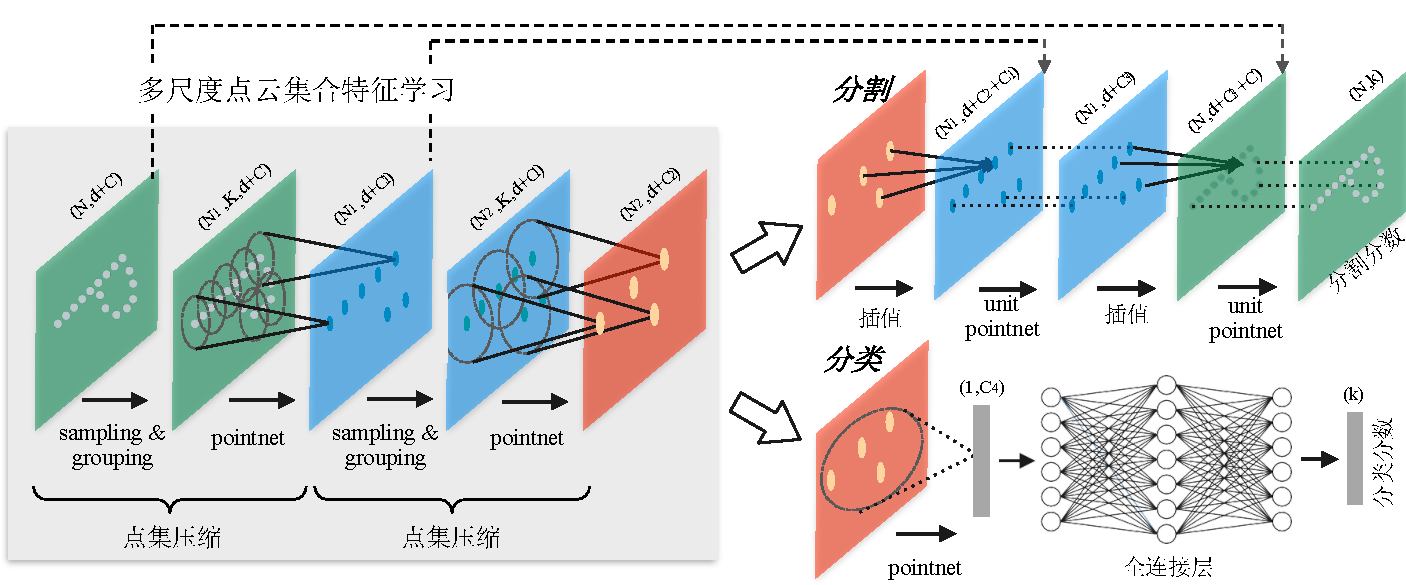
\includegraphics[width=\linewidth]{images/pointnet++.pdf}
    \caption{PointNet++\cite{qi2017pointnet++}网络结构图}
    \label{fig:pointnet++}
    \vspace{-5mm}
\end{figure}

这个方法是受到CNN的启发,在3D点集中找到具有相似结构的子区域,和对应的区域特征embedding,提出了Sampling和Grouping来整合局部邻域的点云,提取局部特征,代码如\ref{lst:pythonfile}。其中,\texttt{farthest point sample}为本段的核心算法,即最远端采样算法来实现从$N$个点中抽取采样$N'$个点。

最远端采样算法 (FPS)的流程如下:
1. 用蒙特卡洛方法筛取初始点,即第0次采样点; \\
2. 计算未采样点与已采样点之间的欧几里得或者推土机距离,将距离最大的点加入已采样点集; \\
3. 更新距离函数,重复1-3,直到获得了目标数量的采样点; \\

\begin{lstlisting}[language=Python, caption={Sampling}, label={lst:pythonfile}]
    def sample_and_group(npoint, radius, nsample, xyz, points, knn=False, use_xyz=True):
    '''
    Input:
        npoint: int32
        radius: float32
        nsample: int32
        xyz: (batch_size, ndataset, 3) TF tensor
        points: (batch_size, ndataset, channel) TF tensor, if None will just use xyz as points
        knn: bool, if True use kNN instead of radius search
        use_xyz: bool, if True concat XYZ with local point features, otherwise just use point features
    Output:
        new_xyz: (batch_size, npoint, 3) TF tensor
        new_points: (batch_size, npoint, nsample, 3+channel) TF tensor
        idx: (batch_size, npoint, nsample) TF tensor, indices of local points as in ndataset points
        grouped_xyz: (batch_size, npoint, nsample, 3) TF tensor, normalized point XYZs
            (subtracted by seed point XYZ) in local regions
    '''
    new_xyz = gather_point(xyz, farthest_point_sample(npoint, xyz)) # (batch_size, npoint, 3)
    if knn:
        _,idx = knn_point(nsample, xyz, new_xyz)
    else:
        idx, pts_cnt = query_ball_point(radius, nsample, xyz, new_xyz)
    grouped_xyz = group_point(xyz, idx) # (batch_size, npoint, nsample, 3)
    grouped_xyz -= tf.tile(tf.expand_dims(new_xyz, 2), [1,1,nsample,1]) # translation normalization
    if points is not None:
        grouped_points = group_point(points, idx) # (batch_size, npoint, nsample, channel)
        if use_xyz:
            new_points = tf.concat([grouped_xyz, grouped_points], axis=-1) # (batch_size, npoint, nample, 3+channel)
        else:
            new_points = grouped_points
    else:
        new_points = grouped_xyz
    return new_xyz, new_points, idx, grouped_xyz
\end{lstlisting}

上面介绍了如何从采样点到局部特征提取的过程,但是在实践中,提取到的不同尺度的特征如何融合对于下游任务的影响也同样很大。PointNet++提出了两种特征融合方式 Multi-Scale Grouping (MSG) 和 Multi-Resolution Grouping (MRG)。如图\ref{fig:pnpp_grouping}(a)、(b)所示。

\begin{figure}[H]
    \vspace{-5mm}
    \centering
    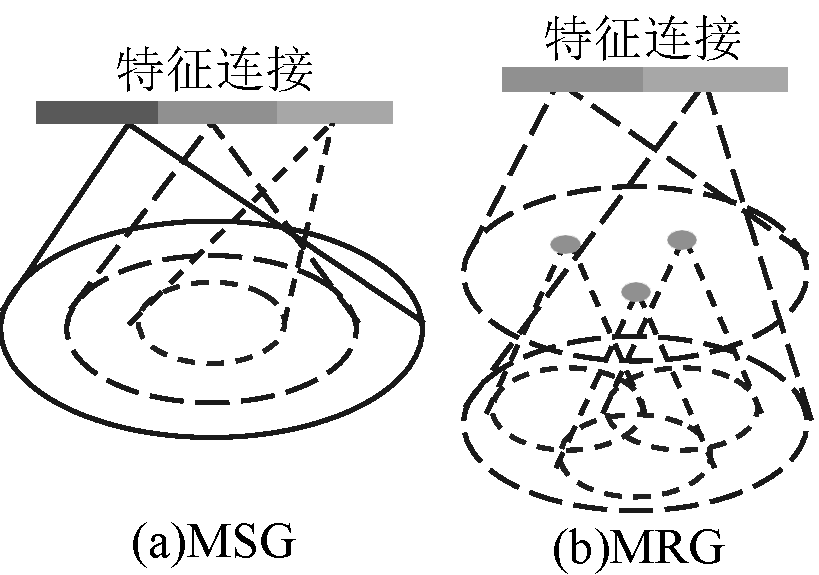
\includegraphics[width=0.45\linewidth]{images/pnpp_group.pdf}
    \caption{多尺度特征融合方法示意图}
    \label{fig:pnpp_grouping}
    \vspace{-25mm}
\end{figure}

对 MSG 方法,具体操作是对不同半径的子区域进行特征提取后进行特征堆叠,特征提取过程还是采用了PointNet,所以对于不同的子区域进行参数计算的时候,使用了不同的网络,计算量过大。对于 MRG 方法来说,使用两个PointNet网络对连续的两层分别做特征提取与聚合,然后再进行特征拼接,可以大大减少参数计算量。

由于PointNet系列网络架构的经典性和鲁棒性,后面的点云处理工作都会借鉴PointNet系列的架构和方法,比如Geometric Transformer\cite{qin2022geometric},采用了PointNet相同的端到端架构,实现了高质量的点云配准;还有PPFNet\cite{deng2018ppf}、PPF-FoldingNet\cite{deng2018ppfnet}、CapsuleNet\cite{sabour2017dynamic}等经典网络,都对该系列进行了借鉴。

\subsection{Predator}

\begin{figure}
    \vspace{-5mm}
    \centering
    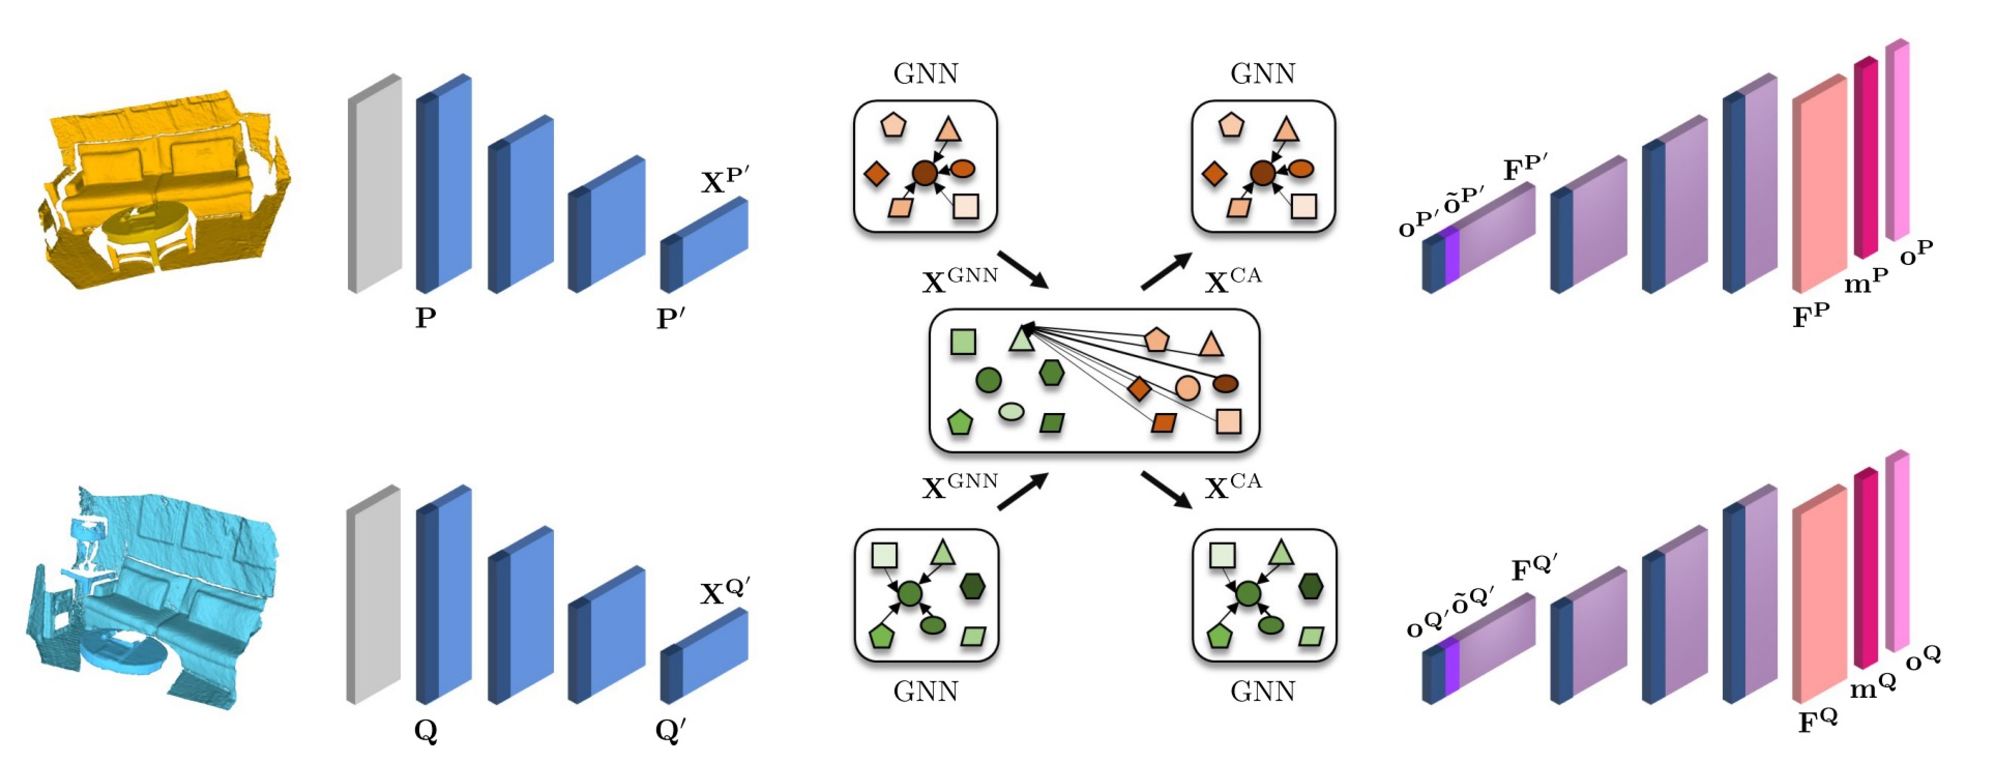
\includegraphics[width=\linewidth]{images/Predator.pdf}
    \caption{
        PREDATOR 的网络结构。体素化的点云 P 和 Q 被送入编码器,它提取出超点 P′ 和 Q′ 及其潜在特征 $\boldsymbol{X_{P'}}$ 和 $\boldsymbol{X_{Q'}}$。重叠注意力模块在一系列自我(GNN)和交叉注意力(Cross Attention)块中,更新特征的共同语境信息,并将它们投影到重叠度 $\boldsymbol{o_{P'}}$、$\boldsymbol{o_{Q'}}$ 和交叉重叠度 $\boldsymbol{\tilde{o}{P'}}$、$\boldsymbol{\tilde{o}{Q'}}$ 的得分。最后,解码器将条件特征和重叠度得分转换为每点特征描述符 $\boldsymbol{F_{P}}$、$\boldsymbol{F_{Q}}$,重叠度得分 $\boldsymbol{o_{P}}$、$\boldsymbol{o_{Q}}$,以及匹配度得分 $\boldsymbol{m_{P}}$、$\boldsymbol{m_{Q}}$。}
    \label{fig:predator}
    \vspace{-5mm}
\end{figure}

Predator\cite{huang2021predator}是一种低重叠度的三维点云配准方法,如图\ref{fig:predator}所示,Predator的架构可以分解为三个主要模块:

1. 将两个点云编码为更小的超点集合和相关的潜在特征编码,权重共享;

2. 重叠注意力模块(在瓶颈中)提取两个点云的特征编码之间的共同语境信息,并为每个超点分配两个重叠得分,这两个得分量化了超点本身和其软对应点位于两个输入之间的重叠区域的可能性;

3. 将相互调节的瓶颈表示解码为点对点描述符以及精化的每点重叠和匹配度得分。

\subsubsection{特征编码}使用大小为 V 的体素网格滤波器对原始点云进行下采样,使得 $\boldsymbol{P}$ 和 $\boldsymbol{Q}$ 具有相当均匀的点密度。在共享编码器中,一系列类似于ResNet的块和跨步卷积将原始点聚合到超点 $\boldsymbol{P' \in R^{N' \times 3}}$ 和 $\boldsymbol{Q' \in R^{M' \times 3}}$,以及相关特征 $\boldsymbol{X_{P'} \in R^{N' \times b}}$ 和 $\boldsymbol{X_{Q'} \in R^{M' \times b}}$。需要注意的是,超点对应于固定的接收场,因此它们的数量取决于输入点云的空间范围,并且对于两个输入可能是不同的。

首先,我们使用大小为 $V$ 的体素网格滤波器对原始点云进行下采样,使得 $\boldsymbol{P}$ 和 $\boldsymbol{Q}$ 具有相当均匀的点密度。在共享编码器中,一系列类似于ResNet的块和跨步卷积将原始点聚合到超点 $\boldsymbol{P' \in R^{N' \times 3}}$ 和 $\boldsymbol{Q' \in R^{M' \times 3}}$,以及相关特征 $\boldsymbol{X_{P'} \in R^{N' \times b}}$ 和 $\boldsymbol{X_{Q'} \in R^{M' \times b}}$。需要注意的是,超点对应于固定的接收场,因此它们的数量取决于输入点云的空间范围,并且对于两个输入可能是不同的。

到目前为止,瓶颈中的特征 $\boldsymbol{X_{P'}}$ 和 $\boldsymbol{X_{Q'}}$ 编码了两个点云的几何形状和上下文。但是,$\boldsymbol{X_{P'}}$ 对点云 Q 一无所知,反之亦然。为了推理它们各自的重叠区域,需要进行一些交叉对话。我们认为,在瓶颈中的超点级别添加这种交叉对话是有意义的,就像人类操作员首先会粗略地了解整体形状以确定可能的重叠区域,然后才会在这些区域中识别出精确的特征点。

图卷积神经网络:在连接两个特征编码之前,我们首先使用图神经网络(GNN)进一步聚合并强化它们各自的上下文关系。首先,使用 k-NN 方法将 $\boldsymbol{P'}$ 中的超点链接成一个欧几里得空间图。设 $\boldsymbol{x_i \in R^b}$ 表示超点 $\boldsymbol{p'_i}$ 的特征编码,$\boldsymbol{(i, j) \in E}$ 表示超点 $\boldsymbol{p'_i}$ 和 $\boldsymbol{p'_j}$ 之间的图边。然后,编码器特征按照以下方式迭代更新:
\begin{equation}
    (k+1)\boldsymbol{x_i} = \max_{(i,j) \in E} h_{\theta} \left[ \text{cat} \left[(k)\boldsymbol{x_i}, (k)\boldsymbol{x_j} - (k)\boldsymbol{x_i} \right] \right]
\end{equation}

这个更新操作执行两次,参数 $\boldsymbol{\theta}$ 并未共享,最终的 GNN 特征 $\boldsymbol{x_{GNN_i} \in R^{d_b}}$ 如下所得:

\begin{equation}
\boldsymbol{x_{GNN_i}} = h_{\theta}(\text{cat}[^{(0)}\boldsymbol{x_i}, ^{(1)}\boldsymbol{x_i}, ^{(2)}\boldsymbol{x_i}])
\end{equation}
其中,$h_{\theta}(·)$ 表示一个线性层,后面跟着实例归一化和 LeakyReLU 激活函数。

上述描述的 GNN 是针对点云 $\boldsymbol{P'}$ 的。对于 $\boldsymbol{Q'}$ 的 GNN 是相同的。

\subsubsection{交叉注意力机制}首先,将点云 $\boldsymbol{P'}$ 中的每个超点连接到 $\boldsymbol{Q'}$ 中的所有超点,形成一个二分图。受到Transformer架构的启发,我们使用向量值查询 $\boldsymbol{s_i \in R^b}$ 来根据其键 $\boldsymbol{k_j \in R^b}$ 检索其他超点的值 $\boldsymbol{v_j \in R^b}$,其中:

\begin{equation}
\begin{aligned}
\boldsymbol{k_j} &= \boldsymbol{W_k x_{GNN_j}} \\
\boldsymbol{v_j} &= \boldsymbol{W_v x_{GNN_j}} \\
\boldsymbol{s_i} &= \boldsymbol{W_s x_{GNN_i}}
\end{aligned}
\end{equation}

这里,$\boldsymbol{W_k}$, $\boldsymbol{W_v}$ 和 $\boldsymbol{W_s}$ 是可学习的权重矩阵。消息计算为值的加权平均,

\begin{figure}
    \vspace{-5mm}
    \centering
    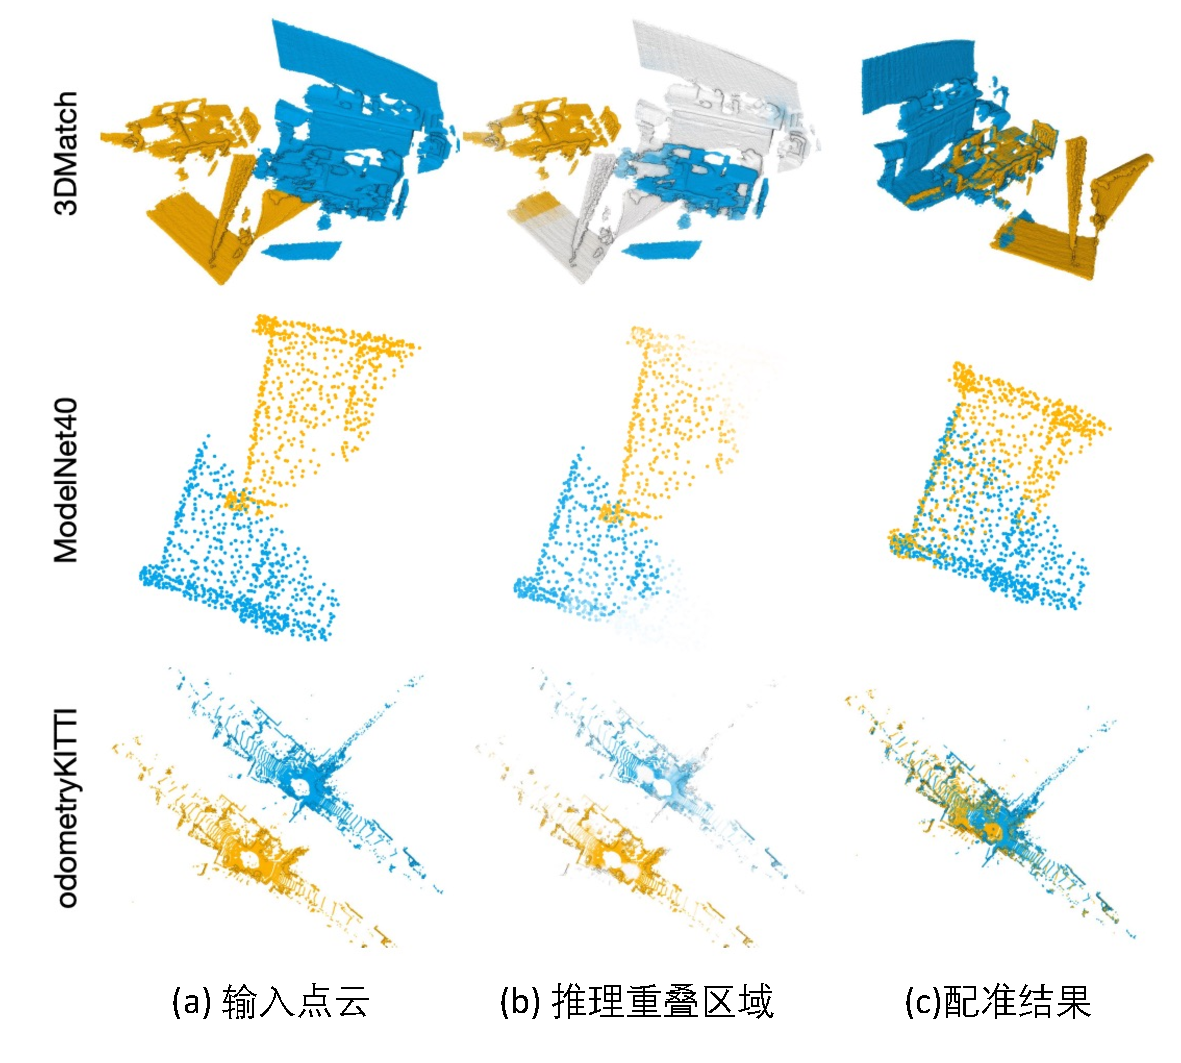
\includegraphics[width=0.6\linewidth]{images/PREDATOR_results.pdf}
    \caption{
        Predator配准示例结果。}
    \label{fig:predator_results}
    \vspace{-5mm}
\end{figure}

\begin{equation}
\boldsymbol{m_{i \leftarrow}} = \sum_{j:(i,j)\in E} a_{ij}\boldsymbol{v_j}
\end{equation}

其中注意力权重 $a_{ij} = \text{softmax}(\boldsymbol{s_i^T k_j}/\sqrt{b})$。也就是说,为了更新超点 $\boldsymbol{p'_i}$,将该点的查询与所有超点 $\boldsymbol{q'_j}$ 的键和值相结合。与文献一致,实际上我们使用具有四个并行注意力头的多注意力层。共同上下文特征计算为

\begin{equation}
\boldsymbol{x_{CA_i}} = \boldsymbol{x_{GNN_i}} + \text{MLP}(\text{cat}[\boldsymbol{s_i}, \boldsymbol{m_{i \leftarrow}}])
\end{equation}

其中 MLP(·) 表示一个三层全连接网络,在第一二层后有实例归一化和ReLU激活函数。相同的交叉注意块也反向应用,使信息在两个方向上流动,$\boldsymbol{P'} \rightarrow \boldsymbol{Q'}$ 和 $\boldsymbol{Q'} \rightarrow \boldsymbol{P'}$。

\subsubsection{瓶颈点的重叠得分}
以上更新共同上下文信息是针对每个超点单独进行的,没有考虑每个点云内的局部上下文。因此,在交叉注意块后,我们使用另一个具有相同架构和底层图(点云内链接)的 GNN 显式更新局部上下文,但参数$\theta$是独立的。这产生了最终的潜在特征编码 $\boldsymbol{F_{P'} \in R^{N' \times b}}$ 和 $\boldsymbol{F_{Q'} \in R^{M' \times b}}$,现在它们是基于其他点云特征的条件。这些特征被线性投影到重叠分数 $\boldsymbol{o_{P'} \in R^{N'}}$ 和 $\boldsymbol{o_{Q'} \in R^{M'}}$,这可以被解释为一个特定超点位于重叠区域的概率。此外,可以计算超点之间的软对应关系,并从对应关系权重预测超点 $\boldsymbol{p'_i}$ 的交叉重叠分数,即其在 $\boldsymbol{Q'}$ 的对应点位于重叠区域的概率:

\begin{equation}
\begin{aligned}
    \label{eq:soft}
\boldsymbol{\tilde{o}{P'i}} & := \boldsymbol{w_i^T o{Q'}}, \
\boldsymbol{w{ij}} & := \text{softmax} \left( \frac{1}{t} \left<\boldsymbol{f_{P'i}}, \boldsymbol{f{Q'_j}}\right> \right),
\end{aligned}
\end{equation}

其中 $\left<\cdot, \cdot\right>$ 是内积,$t$ 是控制软分配的温度参数。在 $t \rightarrow 0$ 的极限下,公式 \ref{eq:soft} 收敛到硬最近邻分配。

\subsubsection{解码器}
我们的解码器从条件特征 $\boldsymbol{F_{P'}}$ 开始,将其与重叠分数 $\boldsymbol{o_{P'}}$ 和 $\boldsymbol{\tilde{o}_{P'}}$ 连接,并输出每点特征描述符 $\boldsymbol{F_P \in R^{N \times 32}}$ 和每点的重叠分数和匹配性得分 $\boldsymbol{o_P, m_P \in R^N}$。匹配性可以被视为“条件显著性”,量化了给定另一个点云 $\boldsymbol{Q}$ 中的点(或特征)时,一个点正确匹配的可能性。

解码器的架构将NN上采样与线性层相结合,并包括来自相应编码器层的跳跃连接。我们有意将重叠得分和匹配性分开,以便解开一个点是好的/坏的匹配候选的原因:原则上,一个点可以被明确地匹配,但位于重叠区域之外,或者它可以位于重叠区域,但具有模糊的描述符。经验上,我们发现网络学习预测高匹配性主要是在重叠区域的点,这可能反映出用于训练的真实对应关系,总是在重叠区域内。结果如图 \ref{fig:predator_results} 所示。

\subsubsection{损失函数}
Predator采用端到端的训练,使用三种与地面真实对应关系相关的损失作为监督。

环形损失:为了监督点特征描述符,我们遵循[3]并使用环形损失[34],这是更常见的三元损失的一种变体。考虑一对重叠点云P和Q,这次与地面真实变换对齐。我们首先提取P中的点$\boldsymbol{p_i} \in \boldsymbol{P_p} \subset \boldsymbol{P}$,该点在Q中至少有一个(可能是多个)对应点,其中对应点集$\boldsymbol{E_p(p_i)}$定义为Q中在$\boldsymbol{p_i}$周围半径$r_p$内的点。同样,Q中所有在半径$r_s$(较大)之外的点形成负面集$\boldsymbol{E_n(p_i)}$。然后从$\boldsymbol{P_p}$中随机抽取$n_p$个点计算环形损失:
\begin{equation}
\boldsymbol{L_P^c} = \frac{1}{n_p} \sum_{i=1}^{n_p} log\left(1 + \sum_{j \in E_p} e^{\beta_j^p(d_j^i - \Delta_p)} \cdot \sum_{k \in E_n} e^{\beta_k^n(\Delta_n - d_k^i)}\right),
\end{equation}
其中$\boldsymbol{d_j^i} = ||\boldsymbol{f_{p_i}} - \boldsymbol{f_{q_j}}||_2$表示特征空间中的距离,$\Delta_n$和$\Delta_p$分别为负面和正面边距。权重$\beta_j^p = \gamma(d_j^i - \Delta_p)$和$\beta_k^n = \gamma(\Delta_n - d_k^i)$分别针对每个正面和负面例子确定,使用经验边距$\Delta_p := 0.1$和$\Delta_n := 1.4$以及超参数$\gamma$。以相同的方式计算反向损失$\boldsymbol{L_Q^c}$,总的环形损失为$\boldsymbol{L_c} = \frac{1}{2} (\boldsymbol{L_P^c} + \boldsymbol{L_Q^c})$。

重叠损失:重叠概率的估计被视为二元分类并使用重叠损失$\boldsymbol{L_o} = \frac{1}{2} (\boldsymbol{L_P^o} + \boldsymbol{L_Q^o})$进行监督,其中
\begin{equation}
\boldsymbol{L_P^o} = \frac{1}{|P|} \sum_{i=1}^{|P|} o_{p_i} log(o_{p_i}) + (1 - o_{p_i}) log(1 - o_{p_i}).
\end{equation}

点$\boldsymbol{p_i}$的地面真实标签$\boldsymbol{o_{p_i}}$定义为
\begin{equation}
\boldsymbol{o_{p_i}} =
\begin{cases}
1, & \text{if } ||\boldsymbol{T_{Q}^{P}(p_i)} - \text{NN}(\boldsymbol{T_{Q}^{P}(p_i)}, Q)||_2 < r_o \\
0, & \text{otherwise},
\end{cases}
\end{equation}
其中$r_o$为重叠阈值。反向损失$\boldsymbol{L_Q^o}$以相同方式计算。正面和负面例子的贡献通过与其相对频率成反比的权重进行平衡。

可匹配性损失:监督可匹配性得分更为困难,因为预先并不清楚在对应关系搜索中应该考虑哪些正确的点。我们遵循一个简单的直觉:好的关键点是那些在训练期间在给定点可以成功匹配的点,使用当前的特征描述符。因此,我们将预测视为二元分类并即时生成地面真实标签。再次,我们将两个对称损失求和,$\boldsymbol{L_m} = \frac{1}{2} (\boldsymbol{L_P^m} + \boldsymbol{L_Q^m})$,其中
\begin{equation}
\boldsymbol{L_P^m} = \frac{1}{|P|} \sum_{i=1}^{|P|} m_{p_i} log(m_{p_i}) + (1 - m_{p_i}) log(1 - m_{p_i}),
\end{equation}
地面真实标签$m_{p_i}$通过在特征空间中进行最近邻搜索NNF(·, ·)即时计算:
\begin{equation}
\boldsymbol{m_{p_i}} =
\begin{cases}
1, & \text{if } ||\boldsymbol{T_{Q}^{P}(p_i)} - \text{NNF}(\boldsymbol{p_i}, Q)||_2 < r_m \\
0, & \text{otherwise}.
\end{cases}
\end{equation}

\section{实验结果与分析}
本文
\subsection{PointNet}
\subsection{PointNet++}
\subsection{Predator}

\section{小结}
本章我们简要介绍了本文所使用的数据集,和点云配准评价指标。然后围绕基于深度学习的点云配准层层递进,由深度学习的基础知识介绍到了目前最常用的深度学习点云处理模型PointNet, PointNet++和Predator。后面,我们会使用预训练的PointNet和Predator作为点云特征提取器,对于描述子进行后处理。